\section{transceiver\_\-mac.c File Reference}
\label{transceiver__mac_8c}\index{transceiver_mac.c@{transceiver\_\-mac.c}}
{\tt \#include $<$inttypes.h$>$}\par
{\tt \#include \char`\"{}transceiver\_\-spi.h\char`\"{}}\par
{\tt \#include \char`\"{}transceiver\_\-mac.h\char`\"{}}\par


Include dependency graph for transceiver\_\-mac.c:\begin{figure}[H]
\begin{center}
\leavevmode
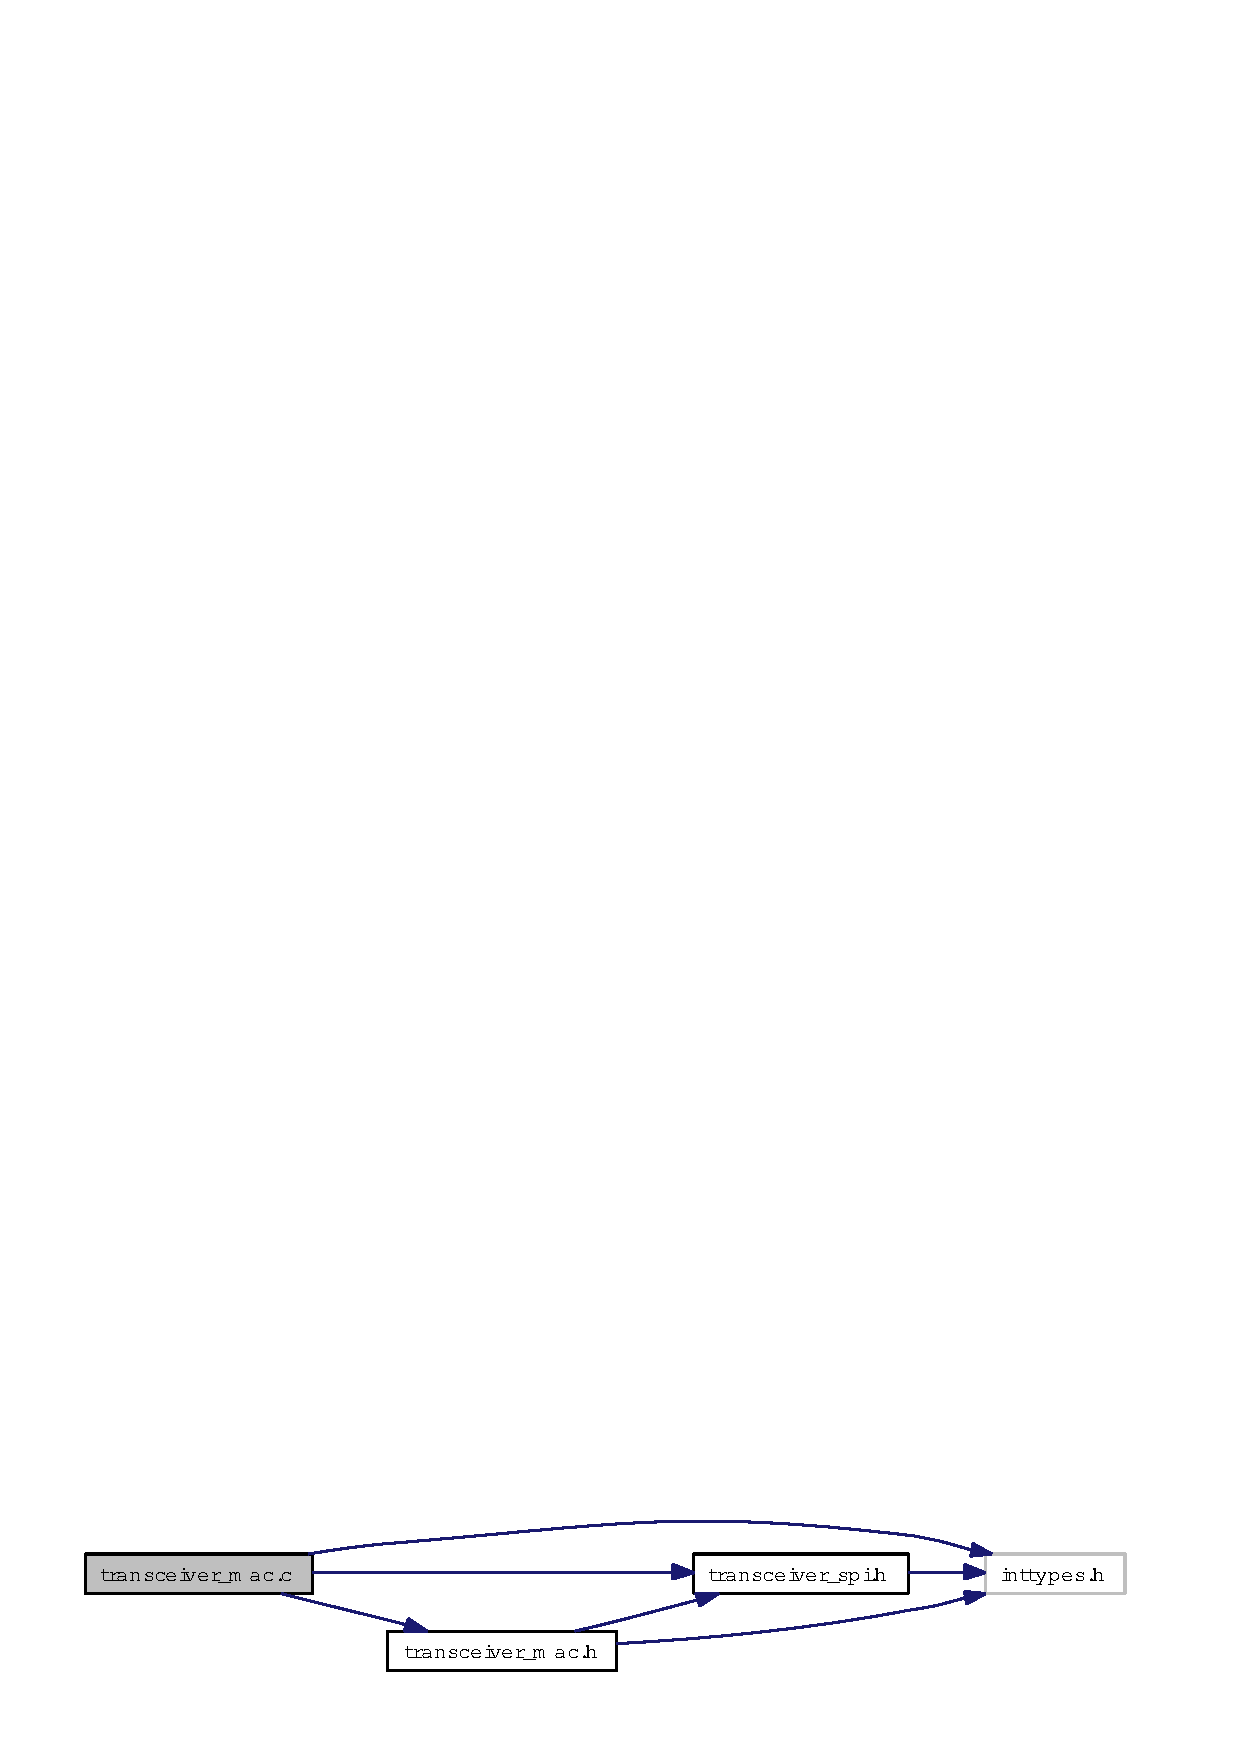
\includegraphics[width=272pt]{transceiver__mac_8c__incl}
\end{center}
\end{figure}
\subsection*{Functions}
\begin{CompactItemize}
\item 
void {\bf MC13192\_\-init} ()
\begin{CompactList}\small\item\em Initialize the MC13192 TODO: write detailed code description! \item\end{CompactList}\item 
void {\bf MC13192\_\-update\_\-state} (void)
\begin{CompactList}\small\item\em Update the state variable to reflect the state of MC13192. \item\end{CompactList}\item 
void {\bf cca\_\-modus} (void)
\item 
void {\bf init\_\-rx\_\-pkt\_\-mode} (void)
\begin{CompactList}\small\item\em switch MC13192 to receive mode TODO: write detailed code description! \item\end{CompactList}\item 
int {\bf get\_\-rx\_\-pkt} ({\bf rx\_\-packet\_\-t} $\ast$rx\_\-packet)
\begin{CompactList}\small\item\em read a data paket from MC13192 \item\end{CompactList}\item 
int {\bf tx\_\-pkt\_\-mode} ({\bf tx\_\-packet\_\-t} $\ast$tx\_\-packet)
\begin{CompactList}\small\item\em send a data packet TODO: write detailed code description! \item\end{CompactList}\end{CompactItemize}
\subsection*{Variables}
\begin{CompactItemize}
\item 
unsigned char {\bf mc13192\_\-mode}
\item 
unsigned char {\bf mc13192\_\-state}
\end{CompactItemize}
